\documentclass[12pt]{report}
\usepackage{graphicx}

\title{SALUTE \\ WEB-BASED MEDICAL MANAGEMENT \\ MILESTONE 0}
\author{Musa Rayyan \\ Nada Hashem \\ Matteo Brucato \\ Ashwin Gopalakrishnan}

\begin{document}
\maketitle
\tableofcontents


\part{Introduction}
Bla bla bla...
\chapter{Overview}
Bla bla bla..
\chapter{Tools and Technology}
What tools and technology we used..


\part{Requirements}
\chapter{User Requirements}
\chapter{System Requirements}
\chapter{Current Status and Future Work}


\part{Design}

\chapter{High Level View}
Bla bla bla..

\section{System Design}
A Web application can be simplified as a collection of resources placed on a server which are accessible to a great number of users (clients). The access to these resources must be governed by policies and permissions. From a very general point of view, our application has two kinds of resources: \emph{public} and \emph{private} resources. For instance, the login page must be a public resource, whereas the setting page should be private.

You can think of a resource as either some data inside a database, a functionality that you ask to your application or even the result of some kind of operation. Based on this view, we decided to use a well-known design approach called MVC (Model-View-Controller) that works very well with this kind of settings. A controller is some executing code that performs exactly the action that the user asked to the server via an URL. In this way, a URL becomes the medium to ask for functionalities and a controller will be a merely executor. A model will be the medium to access data into a database and a view will be a result for the user, in a interface-depending fashion.

In this chapter we will describe our design from a high-level viewpoint, living the implementation for the next chapter.

\section{Database Design}
Bla bla bla... general description ... why we chose to implement it like this... what problems we faced... etc...

\subsection{Entity Relationship Diagram (ERD)}
We provide a high-level description of the database using the famous ER diagram, for those who are familiar with it\footnote{Entities are represented in the ER diagram as rectangles.  Each entity represents a table in the database that holds all of the information or attributes that represents that entity.  In the ER diagram, each attribute is represented with a oval.}. Then we will describe the database structure in more details.

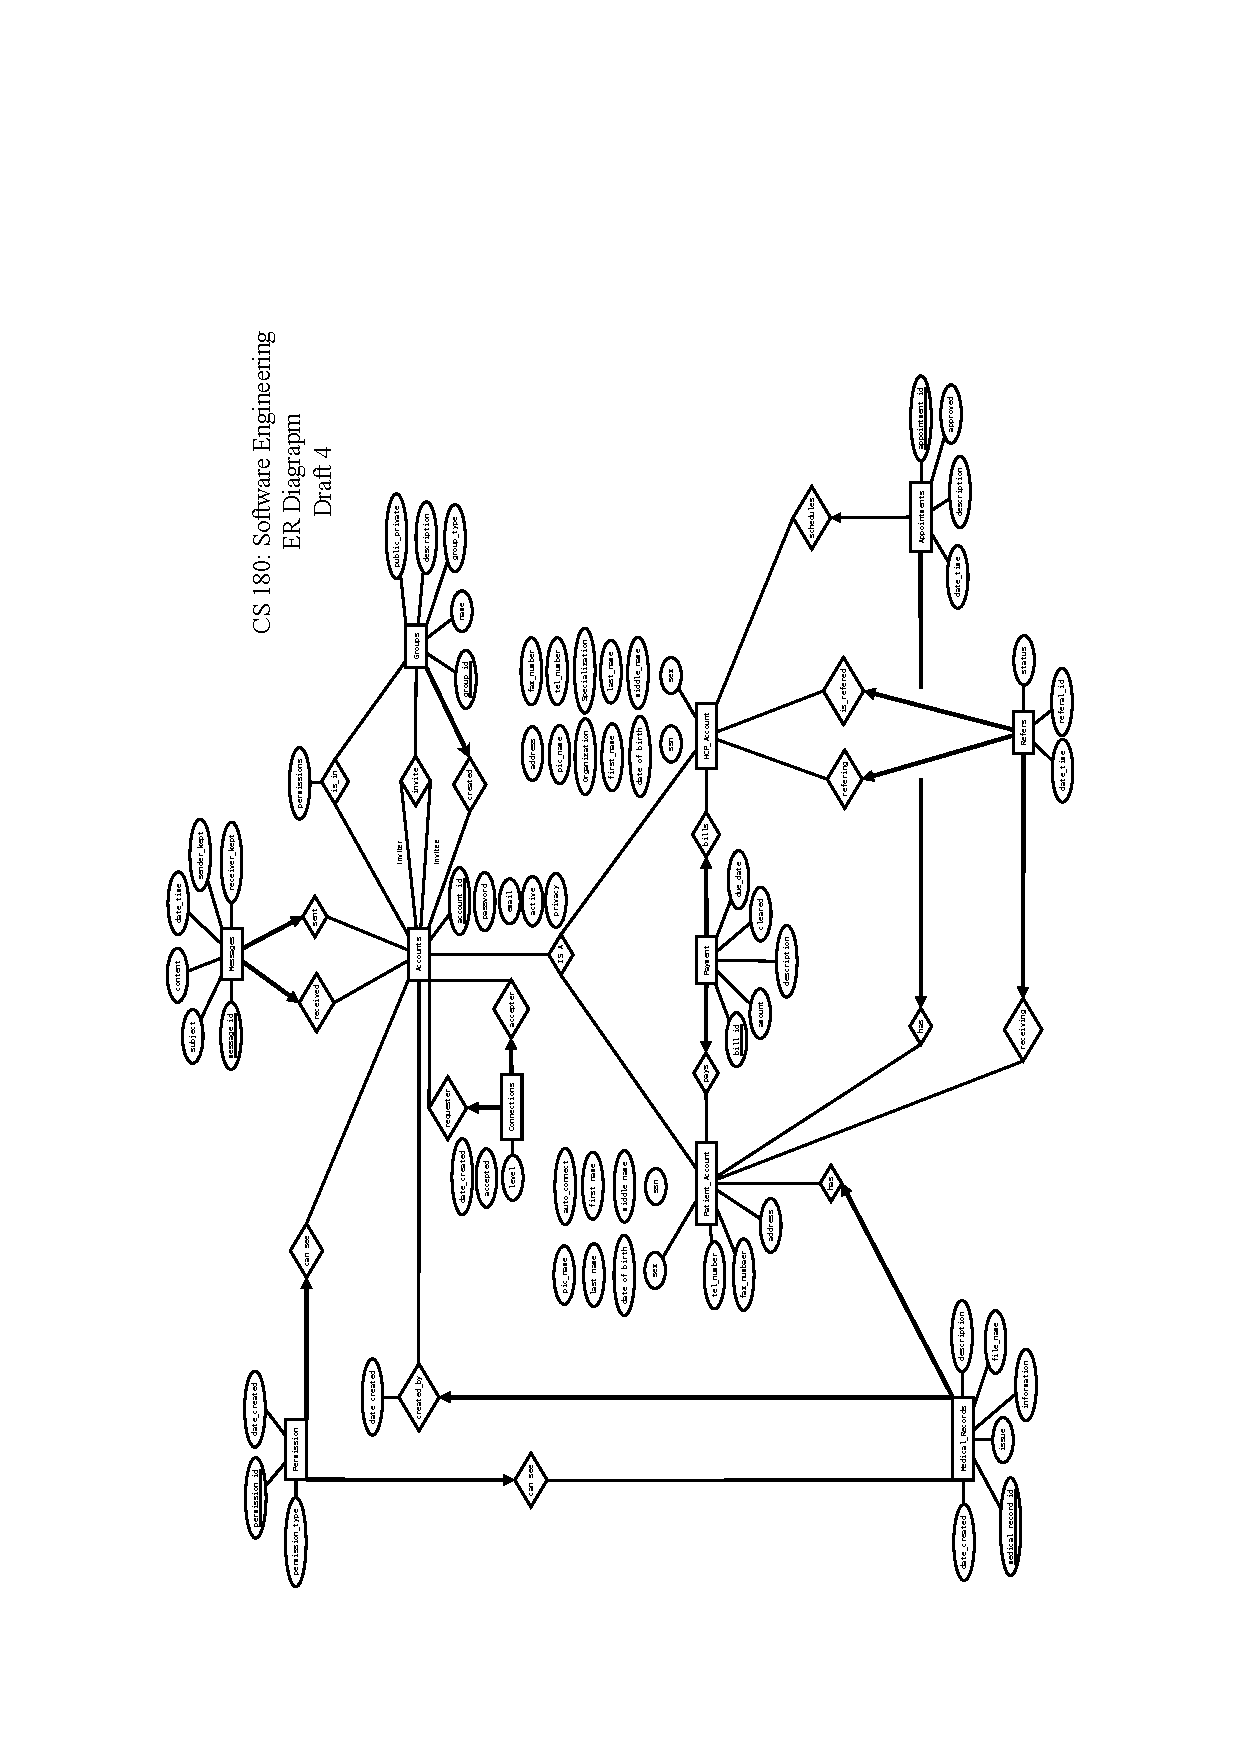
\includegraphics[scale=0.6,angle=180]{cs180_ER_draft4.pdf}

\section{MVC Design}

MVC stands for Model View Controller, and is a software architecture and an architectural pattern in software engineering. The purpose is to separate a system into parts,assigns responsibilities to each, and ensures that they can work together. This design method strives for high cohesion and low coupling which is essential in anticipating for future changes.

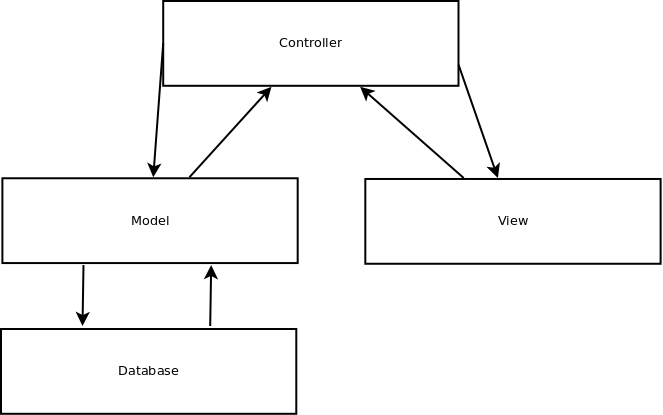
\includegraphics[scale=0.2]{mvc-diag.png}\\
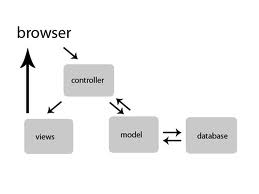
\includegraphics[scale=1]{MVC-Diagram2.jpeg}\\
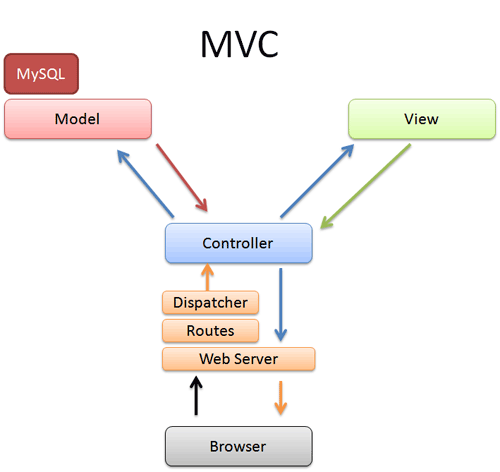
\includegraphics[scale=1]{MVC-Diagram3.png}\\
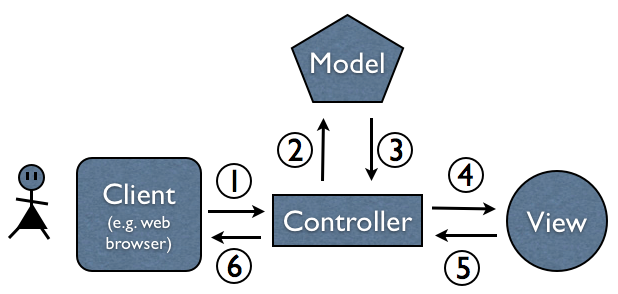
\includegraphics[scale=1]{mvc-diagram4.png}\\
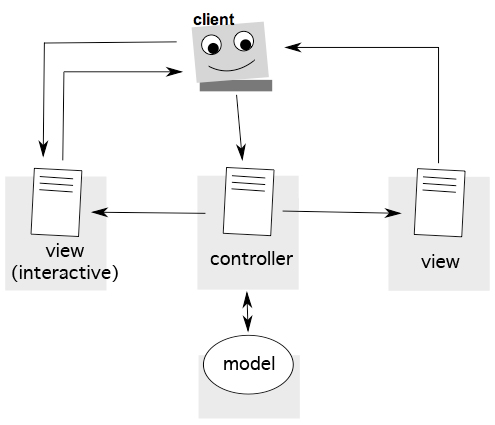
\includegraphics[scale=1]{MVC-Diagram.jpg}\\

\subsection{Models}
The model is the tool used to access and modify the database. Everytime a user needs information, the models are queried to retrieve the information. If a user wants to add or modify, this too must be added into the database. 

\subsection{Views}
The view is the the user interface, what the user sees and interacts with. In our case, its a medical management website. So, it is important to make sure that the website is user-friendly. If the layout and design of the view is difficult to navigate and/or inconsistent, the user will not desire to use the product. 

\subsection{Controllers}
The controller is the middle man. It's in charge of loading the view(webpage) for the user, and calling the corresponding models to execute the functionality that the user has selected via the view. 

\section{Interface Design}
Since this is a Web application, the interface is basically a set of HTML pages that a client gets from the server as it requests them. As for every Web page, the interface is a mixture between different technologies, like HTML, CSS, Javascript and so forth. It is also dependant in some degree by some server features. To keep everything simple, the interface design only defines a very high view of the user system. To allow for a better separation of concerns, we also divided the ''content'' of the Web page from the ''presentation'' of it.
\subsection{UI design}
The GUI is composed by:
\begin{itemize}
\item a header
\item a navigation bar
\item a footer
\item two \emph{dynamic} panels
	\begin{itemize}
	\item a main panel to display the main content of the page
    \item a side panel to display additional information about the main content
	\end{itemize}
\end{itemize}
The header basically contains the branding. The navigation bar allows a user to navigate between all the \emph{public} resources of the entire application and the footer has an extra set of public resources, not directly related to the use of the Web site.

The two panels are \emph{dynamic} in the sense that their content depends on the current resource the user is accessing on a particular moment. They change during the application use, request after request.

\subsection{Ajax}
To follow a generic principle in Software Engineering, we decided to anticipate the change, creating our system capable to do every request using the famous technology Ajax. To be more precise, using requests to server called XMLHTTPRequest. Our interface is ready for that change, and the two dynamic panels are the ones that would change after a XHR request. Both the client and the server are aware of this and whenever the server receives an XHR request, it will answer with only the content for the two dynamic panels. Whereas, if the request is a normal HTTP request, it will provide the whole interface to the client. We will discuss later how we implemented it.

\subsection{Layout}
It's really hard to set a limit between content and presentation in an environment governed by HTML, but something can be done. We created all our views regardless of presentation aspects, focusing only on the most simple aspects of HTML. Our purpose is to separate this two concerns and leave to the \emph{layout} the task to add colours, change positions of the elements and this kind of things. Doing so we also provided the possibility to change the layout in the future, or even dynamically.

\section{Server Design}


\section{Server Design}

\chapter{Implementation View}
[ doxygen here.. ]

\section{Database implementation}
\subsection{Tables}
We will list all the tables... bla bla bla... for each table we will describe all the attributes... bla bla bla...

\subsubsection{Messages}
Holds all of the information regarding messages sent from patient to hcp or vice versa. It has two total 1:N relationships with the Accounts entity.

\begin{description}
\item serial message\_id- ID to uniquely identify the message from other messages. serial datatype automatically creates the message\_id when a new tuple is inserted into the table.  Primary key of the table.  Cannot be null.
\item text subject- Subject of the message being sent. text datatype allows unlimited number of characters.  Cannot be null.
\item text content- Where the sender can writte what they would like to send to the receiver.  text datatype allows unlimited number of characters.  Cannot be null.
\item serial message\_id- ID to uniquely identify the message from other messages. serial datatype automatically creates the message\_id when a new tuple is inserted into the table.  Primary key of the table.  Cannot be null.
\item timestamp date\_time- date and time of when the message is sent.  timestamp datatype format YY:MM:DD HH:MM:SS.  Cannot be null.
\item boolean sender\_kept- To determine if the sender would like to delete the message from their outbox.  boolean value is either true or false.  Cannot be null.  By default it is true.  Changing the status to false means it gets deleted.
\item boolean receiver\_kept- To determine if the receiver would like to delete the message from their inbox.  boolean value is either true or false.  Cannot be null.  By default it is true.  Changing the status to false means it gets deleted.
\end{description}

\subsubsection{Accounts}
Holds all of the primary information every patient and hcp account needs to log into Salute.  The entities Patient\_Account and HCP\_Account both inherit from Accounts using an IS A relationship.  It has a partial N:1 relationship with the Permission and Medical\_Records entities.

\begin{description}
\item serial account\_id- ID to uniquely identify the account from other accounts. serial datatype automatically creates the account\_id when a new tuple is inserted into the table.  Primary key of the table.  Cannot be null.
\item varchar(40) email- Email of the account holder. It is used to log into Salute along with the user password.  varchar(40) datatype allows for a maximum of 40 characters.  Cannot be null.
\item varchar(15) password-  Password of the account holder.  It is used to log into Salute along with the user email address.  varchar(15) datatype allows for a maximum of 15 characters.  Cannot be null.
\item boolean active- To determine wheather the account is active or not.  boolean datatype value is either true or false.  By default it is true.  Changing the stauts to false means the account gets deactivated.
\end{description}

\subsubsection{Patient\_Account}
Holds all of the personal information for every patient.  It inherits from the Accounts entity with an IS A relationship.  It has a partial N:1 relationship with the Medical\_Records entity and a partial N:M relationship with the p\_d\_connection relationship.

\begin{description}
\item serial account\_id- ID to uniquely identify the account from other accounts. serial datatype automatically creates the account\_id when a new tuple is inserted into the table.  This ID is inherited from the Accounts entity. Primary key of the table.  Cannot be null.
\item varchar(30) first\_name-  First name of the patient.  varchar(30) datatype allows for a maximum of 30 characters.  Cannot be null.
\item varchar(30) last\_name- Last name of the patient.  varchar(30) datatype allows for a maximum of 30 characters.  Cannot be null.
\item varchar(30) middle\_name- Middle name of the patient. varchar(30) datatype allows for a maximum of 30 characters.
\item numeric(9,0) ssn- Social Security Number of the patient. numeric(9,0) datatype allows exactly 9 numeric characters.  Cannot be null.
\item date dob- date of Birth of the patient.  date datatype is of the format YY:MM:DD.  Cannot be null.
\item char(6) sex- Sex of the patient. char(6) datatyep allows for a maximum of 6 characters.  It has to be either "male" or "female".  Cannot be null.
\item varchar(11) tel\_number- Primary telephone number of the patient.  varchar(11) datatype allows a maximum of 11 characters.
\item varchar(11) fax\_number- Fax number of the patient.  varchar(11) datatype allows a maximum of 11 characteres.
\item text address- Primary address of the patient.  text datatype allows unlimited number of characters.
\end{description}

\subsubsection{HCP\_Account}
Holds all of the personal information for every hcp.  It inherits from the Accounts entity with an IS A relationship.  It has a partial N:1 relationship with the Appointments and Payment entities, as well as a partial N:M relationship with the p\_d\_connection and d\_d\_connection relationship.

\begin{description}
\item serial account\_id- ID to uniquely identify the account from other accounts. serial datatype automatically creates the account\_id when a new tuple is inserted into the table.  This ID is inherited from the Accounts entity. Primary key of the table.  Cannot be null.
\item varchar(30) first\_name-  First name of the hcp.  varchar(30) datatype allows for a maximum of 30 characters.  Cannot be null.
\item varchar(30) last\_name- Last name of the hcp.  varchar(30) datatype allows for a maximum of 30 characters.  Cannot be null.
\item varchar(30) middle\_name- Middle name of the hcp. varchar(30) datatype allows for a maximum of 30 characters.
\item numeric(9,0) ssn- Social Security Number of the hcp. numeric(9,0) datatype allows exactly 9 numeric characters.  Cannot be null.
\item date dob- date of Birth of the hcp.  date datatype is of the format YY:MM:DD.  Cannot be null.
\item char(6) sex- Sex of the hcp. char(6) datatyep allows for a maximum of 6 characters.  It has to be either "male" or "female".  Cannot be null.
\item varchar(11) tel\_number- Primary office telephone number of the hcp.  varchar(11) datatype allows a maximum of 11 characters.
\item varchar(11) fax\_number- Primary fax number of the hcp.  varchar(11) datatype allows a maximum of 11 characteres.
\item text specialization- What the hcp specializes in.  text datatype allows unlimited number of characters.
\item varchar(30) org\_name- Name of the organization for which the hcp works for.  varchar(30) datatype allows a maximum of 30 characteres.
\item text address- Primary address of the hcp place of business.  text datatype allows unlimited number of characters.
\end{description}

\subsubsection{Appointments}
Holds all of the information for every appointment a patient makes with a hcp.  It has a total 1:N relationship with the HCP\_Account and Patient\_Account entities.

\begin{description}
\item serial appointment\_id- ID to uniquely identify the appointment from other appointments. serial datatype automatically creates the appointment\_id when a new tuple is inserted into the table.  Primary key of the table.  Cannot be null.
\item serial patient\_id-  Unique account ID of the patient that requests the appointment.  This is the foreign key to the Patient\_Account entity.  Cannot be null.
\item serial hcp\_id- Unique account ID of the hcp that receives the appointment request.  This is the foreign key to the HCP\_Account entity.  Cannot be null.
\item text descryption- Description of the appointment that the patient requests to the hcp.  text datatype allows unlimited number of characters.  Cannot be null.
\item timestamp date\_time- Time and day of the appointment the patient requestes to the hcp.  timestamp datatype of the form YY:MM:DD HH:MM:SS.  Cannot be null.
\item boolean approved- Status of the appointment that the patient requests to the hcp.  boolean datatype value is either true or false.  By default it is false.  HCP can accept the appointment and change the status to true.
\end{description}

\subsubsection{Medical\_Record}
Holds all of the information for every medical record a patient has on Salute.  It has a partial N:1 relationship with the Permission entity and a total 1:N relationship with the Accounts and Patient\_Account entities.

\begin{description}
\item serial medical\_rec\_id- ID to uniquely identify the medical record from other medical records. serial datatype automatically creates the medical\_rec\_id when a new tuple is inserted into the table.  Primary key of the table.  Cannot be null.
\item serial patient\_id- Unique account ID of the patient that owns the medical record.  This is the foreign key to the Patient\_Account entity.  Cannot be null.
\item serial account\_id- Unique account ID of the user(patient/hcp) that uploads the medical record.  This is the foreign key to the Accounts entity.  Cannot be null.
\item text issue-  What the medical record deals with.  text datatype allows unlimited number of characters.  Cannot be null.
\item text suplementary\_info- Any suplementary infomation that anybody (patient/hcp) would want to add to the medical record.  text datatype allows unlimited number of characters.
\item text file\_path- Path where the file can be found and downloaded from the server.  text datatype allows unlimited number of characters.  Cannot be null.
\end{description}

\subsubsection{Payment}
Holds all of the information for every bill that a patient receives and a hcp issues.  It has a total 1:N relationship with the Patient\_Account and HCP\_Account entities.

\begin{description}
\item serial bill\_id serial-  ID to uniquely identify the bill from other bills. serial datatype automatically creates the bill\_id when a new tuple is inserted into the table.  Primary key of the table.  Cannot be null.
\item serial patient\_id- Unique account ID of the patient that received the bill.  This is the foreign key to the Patient\_Account entity.  Cannot be null.
\item serial hcp\_id- Unique account ID of the hcp that issued the bill.  This is the foreign key to the HCP\_Account entity.  Cannot be null.
\item decimal(9,2) amount- The amount due to the hcp.  decimal datatype allows charge to be up to 9 digits long, with 2 digits of percision.  Cannot be null.
\item text descryption- Descryption of what the bill is being issued for.  text datatype allows unlimited number of characters. Cannot be null.
\item timestamp due\_date- date by which the bill must be paid by.  timestamp datatype of the form YY:MM:DD HH:MM:SS.  Cannot be null.
\item boolean cleared- States wheather the bill was paid or not.  boolean datatype value is either true or false.  By default it is false.  If patient pays the bill, its status is changed to true.
\end{description}

\subsubsection{Permission}
Holds information regarding which medical records a hcp that is connected with a patient can view.  It has a total 1:N relationship with the Accounts and Medical\_Records entities.

\begin{description}
\item serial permission\_id-  ID to uniquely identify the permission from other permissions. serial datatype automatically creates the permission\_id when a new tuple is inserted into the table.  Primary key of the table.  Cannot be null.
\item medical\_rec\_id- Unique ID of the medical record that a hcp can view.  This is the foreign key to the Medical\_Records entity.  Cannot be null.
\item serial account\_id- Unique ID of the hcp that can view the medical record.  This is a foreign key to the Accounts entity.  Cannot be null.
\item date date\_created-  date in which the patient allowed the hcp to view the medical record.  date datatype is of the form YY:MM:DD.  Cannot be null.
\end{description}

\subsubsection{p\_d\_connection}
Holds all of the information for every connection between a patient and a hcp.  This relationship has a patial N:M relationship with the HCP\_Account and the Patient\_Account entities.

\begin{description}
\item serial patient\_id- Unique account ID of the patient that establishes a connection with a hcp.  The combination of patient\_id and hcp\_id is the primary key for this table.  This is also the foreign key to the Patient\_Account entity.  Cannot be null.
\item serial hcp\_id- Unique account ID of the hcp that accepts the connection request sent from the patient.  The combination of hcp\_id and patient\_id is the primary key for this table.  This is also the foreign key to the HCP\_Account entity.  Cannot be null.
\item boolean accepted- States wheather the request was accepted by the hcp.  boolean datatype value is either true or false.  By default it is false.  If hcp accepts the request, its status is changed to true.
\item date date\_connected- date in which the request was sent by the patient to the hcp.  date datatype is of the form YY:MM:DD.  Canot be null.
\end{description}

\subsubsection{d\_d\_connection}
Holds all of the information for every connection between a hcp and another hcp.  This relationship has two patial N:M relationships with the HCP\_Account entity.

\begin{description}
\item serial requester\_id- Unique account ID of the hcp that establishes a connection with another hcp.  The combination of requester\_id and accepter\_id is the primary key for this table.  This is also a foreign key to the HCP\_Account entity.  Cannot be null.  
\item serial accepter\_id- Unique account ID of the hcp that accepts the connection request sent from hcp.  The combination of accepter\_id and requester\_id is the primary key for this table.  This is also a foreign key to the HCP\_Account entity.  Cannot be null.
\item boolean accepted- States wheather the request was accepted by the hcp.  boolean datatype value is either true or false.  By default it is false.  If hcp accepts the request, its status is changed to true.
\item date date\_connected- date in which the request was sent by the hcp to the other hcp.  date datatype is of the form YY:MM:DD.  Canot be null.
\end{description}

\subsubsection{Scripts to start the server and load the data}
We used many scripts to create the database described above.  First of all we have a bash script called start\_everything.sh which as its name implies, starts everything.  It starts the PostgreSQL server, creates a PostgreSQL database, and then it uses an sql file called create\_tables.sql to create all of the tables described in the ER diagram.  It then calls the file load\_data.sql which loads all of the tables with test data.  In case we want to drop all of the test data we have an sql file called drop.sql.  In case we wanted to delete everything and start over, we have a bash script called delete\_everything.sh. 

\section{MVC implementation}
[ doxygen here... ]

\subsection{Assumptions}
\begin{itemize}
\item Doctors cannot delete medical records even if they uploaded them, only patients can
\item Both doctors and patients can upload medical records
\item When a doctor uploads a medical record, he has automatic viewing priveleges
\item doctors cannot request appointments
\item patients cannot accept an appointment
\item doctors aren't allowed to reschedule an appointment
\item both doctors and patients can cancel an appointment
\end{itemize}

\section{Interface implementation}
\subsection{Layouts}
Client-side and server-side... how the interface design is handled in the server and how XHTML and CSS are used to provide the interface. Talk about class "Layout" server-side.
\subsection{JQuery}
Give fancy effects... handle Ajax... 
\subsection{Ajax interaction between client and server}
Talk about class="ajaxlink" and JQuery triggers. Talk about class "Ajax" server-side.

\section{Tests}

\subsection{Controller Tests}

There are three types of users: non-members, patients, and health care providers. Each type have been tested individually.

A non-member should only be able to view the default home page, or register. All other functions were tested to assure that a non-member could not access any other functionalities. 

A patient is able to do the following:
\begin{itemize}
\item Login, Logout
\item Requesting a connection with a healthcare provider
\item Delete a connection with their healthcare provider
\item Viewing all, pending, or connected healthcare providers
\item Viewing their medical records
\item Make an appointment with a connected doctor
\item Cancel an appointment 
\item View all,upcoming, or past appointments
\item Change their email, or password
\item Retrieve their password if forgotten via email
\item Edit their information
\item Deactivate, reactivate their account
\item View all, current, or past bills.
\item Pay their bills (Note: This is not linked to any credit card/bank system ) 
\item Add or delete a medical record
\item View all their medical records
\item Set each medical record to hidden or public to specific healthcare providers
\item Send a message to doctors
\end{itemize}
A health care provider is able to do the following:
\begin{itemize}
\item Login, Logout
\item Requesting a connection with a healthcare provider
\item Accept a connection request from another health care provider or patient
\item Reject a connection request from another health care provider or patient
\item Delete a connection with their patient or collegue
\item Viewing all healthcare providers
\item Viewing pending incoming requests with other healthcare providers
\item Viewing pending outgoing requests with other healthcare providers
\item Viewing connected collegues, and patients
\item Accept a requested appointment from their patients
\item Cancel an existing appointment
\item View all,upcoming, and past appointments
\item Change their email or password
\item Retrieve their password if forgotten via email
\item Edit their information
\item Deactivate, and reactivate their account
\item View all, current, or past bills.
\item Issue bills to connected patients
\item Add a medical record to a specific patient
\item Viewing their patient's medical records (the ones they are authorized to see)
\item Set each medical record to hidden or public to specific healthcare providers
\item Send a message their patients or collegues

\end{itemize}

\subsection{Database Tests}

\part{Operating Manual}
\chapter{How-to's}
\chapter{Registration and login}
\chapter{Viewing a user profile}
\chapter{Connection management}

\chapter{Screen-shots}

\part{Credits}


\end{document}
